\section{Metodo}

In questa sezione viene descritto l'approccio adottato per risolvere il problema, formulato come task di classificazione in quattro categorie (indicazione, pericolo, divieto, background).

\subsection{Rete Utilizzata}

In seguito a una fase preliminare di sperimentazione (discussa nel capitolo successivo), è stata selezionata una Convolutional Neural Network (CNN) ispirata ad AlexNet, denominata \textit{LeNetColor}. L'architettura è stata progressivamente migliorata mediante l'introduzione di \textit{Batch Normalization} e \textit{Dropout}, al fine di stabilizzare l'addestramento e ridurre il rischio di overfitting. Nel seguito, il modello finale viene indicato come \textbf{MiniAlexNetV2}. La Figura \ref{fig:reti} mostra la rete di partenza (\textit{LeNetColor}) e la sua prima evoluzione (\textit{MiniAlexNet}), mentre la Figura \ref{MiniAlexNetV2} riporta l'architettura finale selezionata.

\begin{figure}[htbp]
\centering
\begin{minipage}[t]{0.50\textwidth}
    \centering
    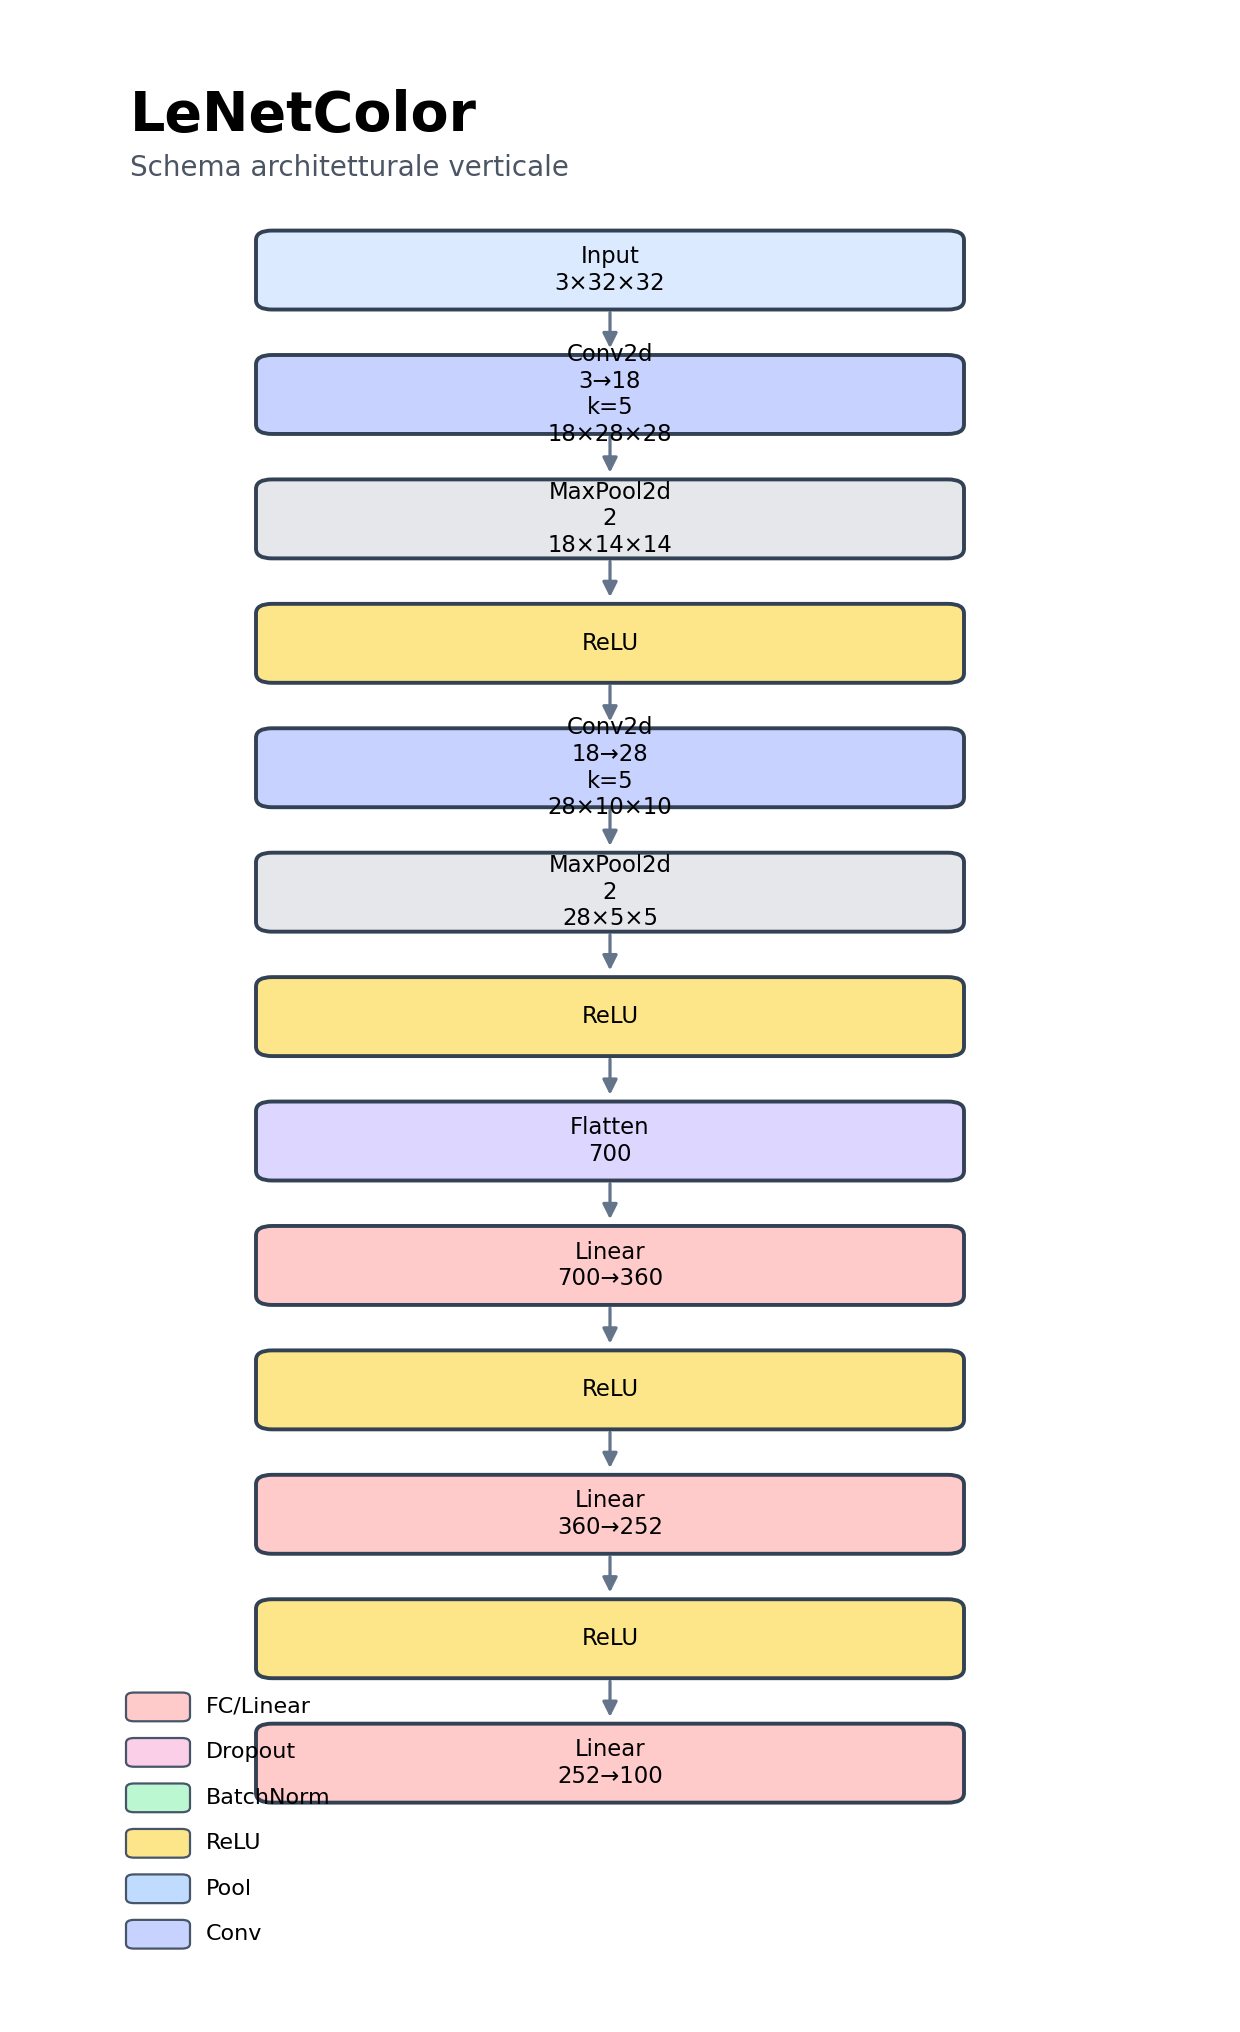
\includegraphics[width=\linewidth]{Metodo/LeNetColor_vertical.png}
\end{minipage}\hfill
\begin{minipage}[t]{0.50\textwidth}
    \centering
    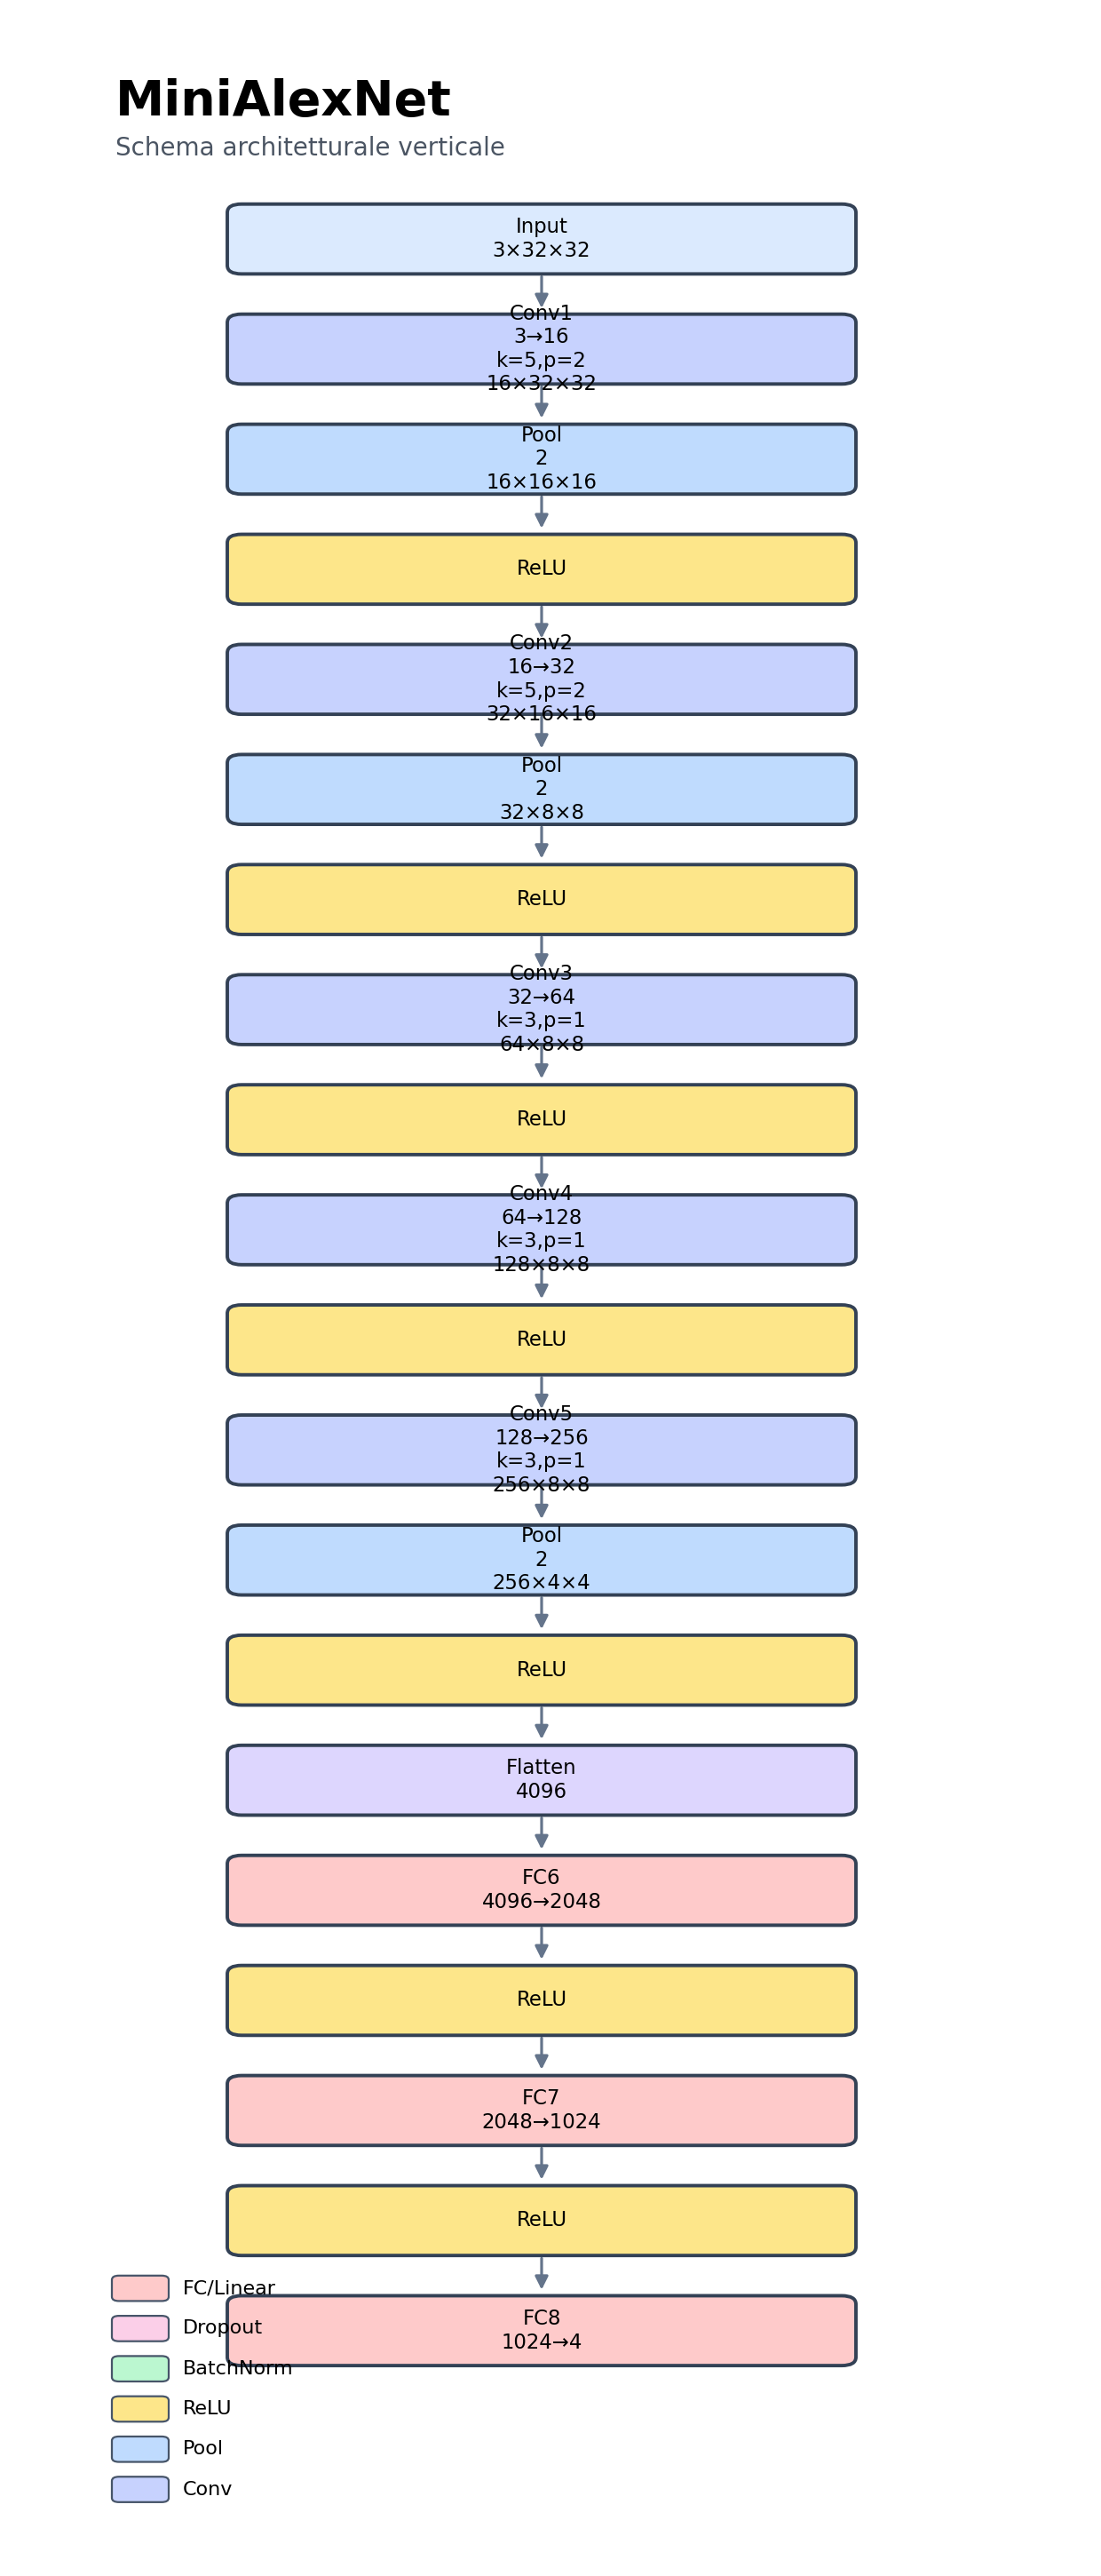
\includegraphics[width=\linewidth]{Metodo/MiniAlexNet_vertical.png}
\end{minipage}\hfill

\caption{Confronto tra LeNetColor e MiniAlexNet}
\label{fig:reti}
\end{figure}

\begin{figure}
    \centering
    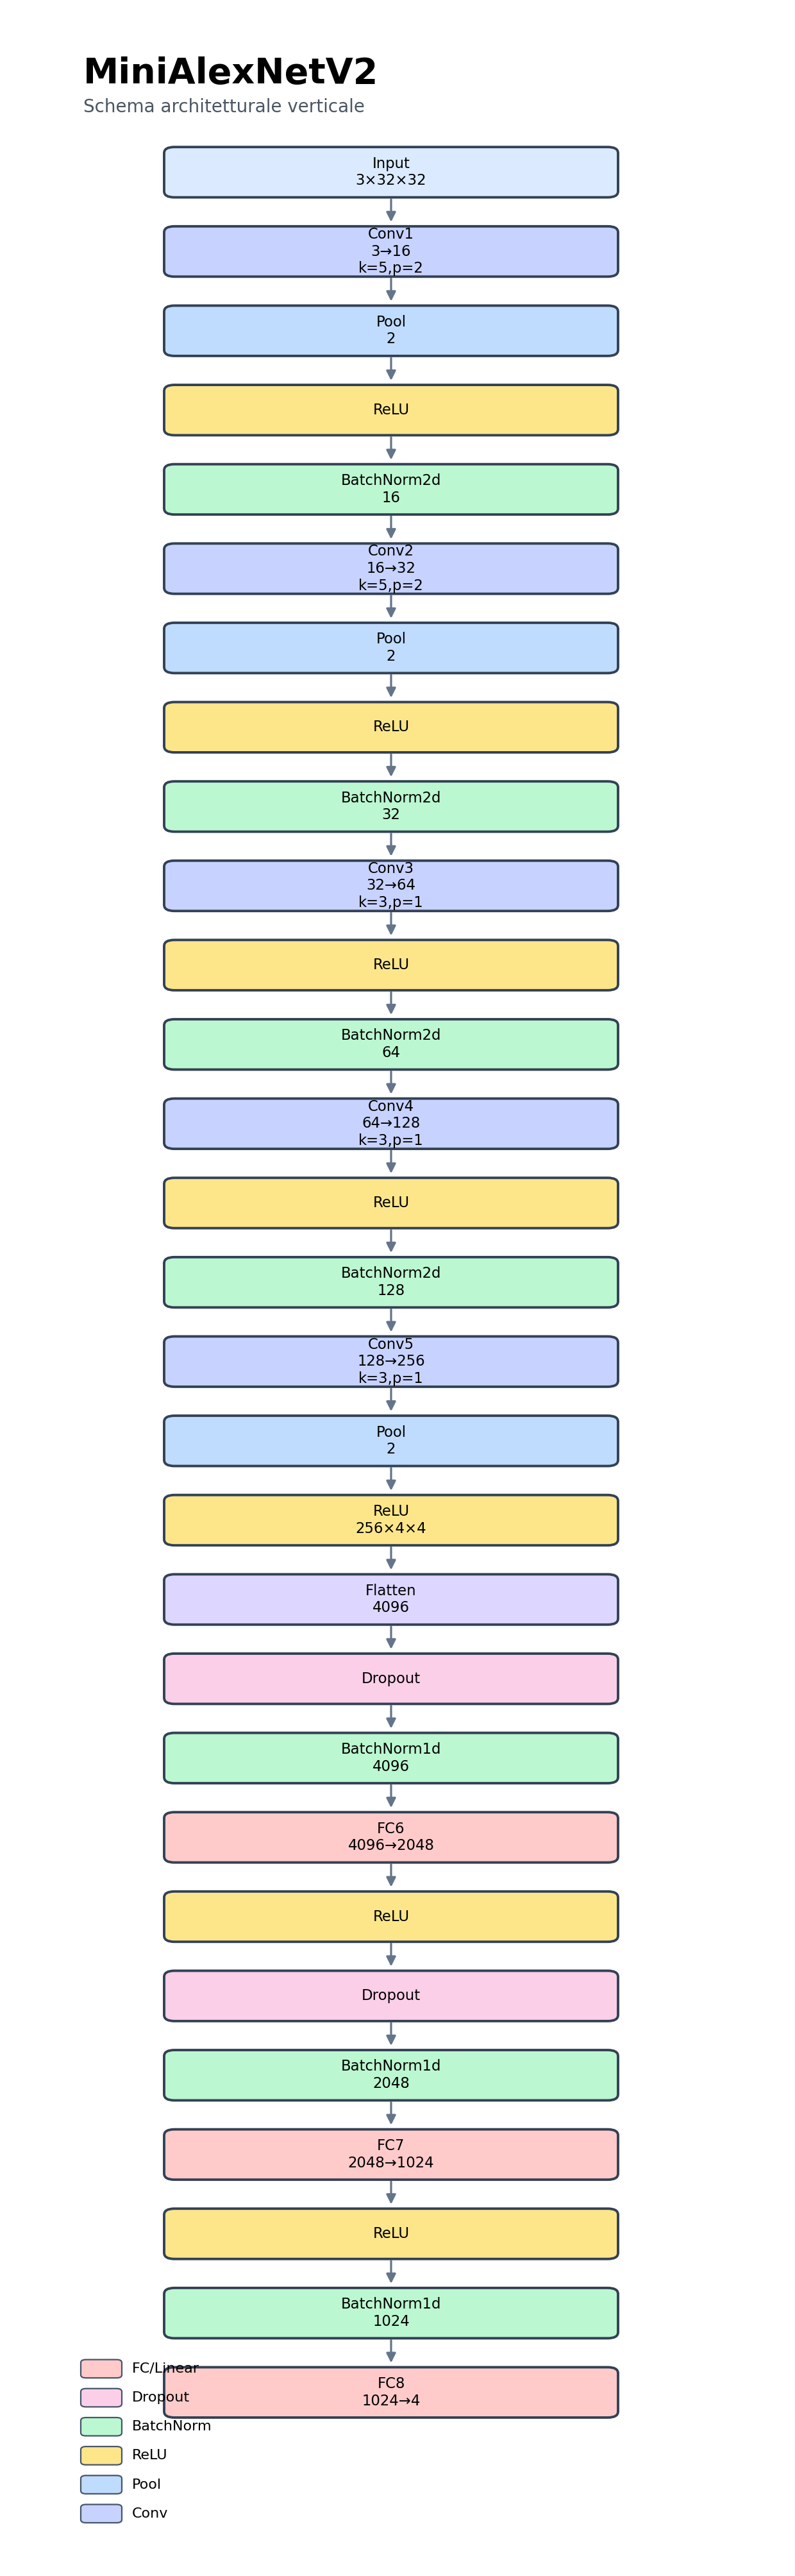
\includegraphics[scale=0.4]{Metodo/MiniAlexNetV2_vertical.png}
    \caption{MiniAlexNetV2, rete utilizzata per il training}
    \label{MiniAlexNetV2}
\end{figure}

Per la configurazione di input sono state adottate scelte empiriche consolidate: batch size pari a 1024 in addestramento e 2048 in validazione/test, con strati di MaxPooling (kernel 2, stride 1). Come funzione di attivazione è stata utilizzata la Rectified Linear Unit (ReLU), che annulla i valori negativi e mantiene invariati i valori positivi. Tale funzione è descritta in \eqref{1}:

\begin{equation}
    f(x) = \begin{cases}
                0 & \text{se } x < 0 \\
                x & \text{se } x > 0
           \end{cases}
\label{1}
\end{equation}

\subsection{Funzione di Loss}
La funzione di loss adottata è la \textit{Cross Entropy Loss}, riportata in \eqref{2}:

\begin{equation}
    \text{Cross Entropy Loss} = -\frac{1}{N} \sum_{i=1}^{N} \sum_{j=1}^{C} y_{ij} \cdot \log(\hat{y}_{ij})
\label{2}
\end{equation}

dove:
\begin{align*}
    N & \text{ è il numero di campioni,} \\
    C & \text{ è il numero di classi,} \\
    y_{ij} & \text{ è la vera probabilità della classe } j \text{ per il campione } i, \\
    \hat{y}_{ij} & \text{ è la probabilità predetta della classe } j \text{ per il campione } i.
\end{align*}

La cross entropy loss consente di confrontare due distribuzioni di probabilità: quella predetta dal modello e quella target. Nel caso in esame, \textbf{MiniAlexNetV2} produce per ciascuna immagine una distribuzione di probabilità sulle classi, che viene confrontata con la distribuzione reale.

In termini operativi, è stata inoltre considerata la seguente variante della funzione di loss:

\begin{equation}
    \text{Cross Entropy Loss} = -\frac{1}{N}\sum_{i}^{N} \left( y_i \cdot \log(\hat{y}_i) + (1 - y_i) \cdot \log(1 - \hat{y}_i) \right)
\label{3}
\end{equation}

dove:
\begin{align*}
    N & \text{ è il numero di classi,} \\
    y_i & \text{ è la vera probabilità della classe } i, \\
    \hat{y}_i & \text{ è la probabilità predetta della classe } i.
\end{align*}

\subsection{Valutazione}
La qualità delle previsioni è stata valutata tramite il parametro di accuratezza, derivato a partire da una matrice di confusione elementare (Tabella \ref{tab:matrice-confusione}):

\begin{table}[H]
\centering
\begin{tabular}{|c|c|c|}
\hline
\multirow{2}{*}{} & \multicolumn{2}{c|}{\cellcolor{gray!20}\textbf{Realtà}} \\ \cline{2-3}
 & \cellcolor{gray!20}\textbf{Positivo} & \cellcolor{gray!20}\textbf{Negativo} \\ \cline{1-3}
\cellcolor{gray!20}\textbf{Previsione Positiva} & \cellcolor{green!20}Vero Positivo & \cellcolor{red!20}Falso Positivo \\ \cline{1-3}
\cellcolor{gray!20}\textbf{Previsione Negativa} & \cellcolor{red!20}Falso Negativo & \cellcolor{green!20}Vero Negativo \\ \cline{1-3}
\end{tabular}
\caption{Matrice di Confusione}
\label{tab:matrice-confusione}
\end{table}

\vspace{+1truecm}

L'accuratezza del modello è definita come rapporto tra il numero di previsioni corrette e il numero totale di previsioni, come espresso in \eqref{4}:
\begin{equation}
\text{Accuracy} = \frac{\text{Numero di Previsioni Corrette}}{\text{Numero Totale di Previsioni}}
\label{4}
\end{equation} 
\newline

Tale parametro fornisce una misura sintetica della capacità di classificazione del modello.
\newline 
Accanto all'accuratezza è stata analizzata anche la curva ROC, che descrive l'andamento delle prestazioni al variare della soglia decisionale.






